\documentclass[11pt,a4paper]{article}

\usepackage[T1]{fontenc}
\usepackage[utf8]{inputenc}
\usepackage[polish]{babel}
\usepackage{amsmath,amssymb}
\usepackage{graphicx}
\usepackage{booktabs}
\usepackage{url}
\usepackage{hyperref}

\hypersetup{
  colorlinks=true,
  linkcolor=blue,
  urlcolor=blue,
  citecolor=blue
}

\title{Symulacja drapieżnik--ofiara z uczeniem ze wzmocnieniem\\(implementacja wg Park et al., 2021)}
\author{---}
\date{\today}

\begin{document}
\maketitle

\begin{abstract}
\textit{[Streszczenie całej pracy --- do uzupełnienia po napisaniu wstępu i części porównawczej.]}
\end{abstract}

% --------------------------------------------------------------------------
\section{Inne podejścia do problemu}
\label{sec:inne-podejscia}

\textit{[Tu: opis wcześniejszych lub alternatywnych podejść do modelowania dynamiki drapieżnik--ofiara --- literatura, prostsze modele, inne metody RL itp. Fragment do uzupełnienia.]}

\subsection*{Szkic podsekcji (opcjonalnie)}
\textit{[Do uzupełnienia.]}

% --------------------------------------------------------------------------
\section{Implementacja według Park et al.\ (2021)}
\label{sec:park}

Niniejsza część opisuje środowisko, uczenie i wyniki zgodne z pracą Park et al.~\cite{park2021}, w powiązaniu z modułami \texttt{park\_env} oraz \texttt{park\_train} w repozytorium projektu.

\subsection{Środowisko symulacyjne}
\label{sec:srodowisko}

Świat jest dyskretną siatką \(N \times N\) komórek (domyślnie \(N=50\)). W każdej komórce może znajdować się co najwyżej jeden agent (drapieżnik lub ofiara). Granice są \emph{okresowe} (torus): ruch i obserwacja lokalna zawijają się modulo \(N\), analogicznie do założeń w~\cite{park2021}. Agenci nie komunikują się jawnie.

\textbf{Inicjalizacja epizodu.} Losowa permutacja komórek; następnie rozmieszczenie \(n_X=100\) drapieżników i \(n_Y=500\) ofiar na pustych polach. Wartości domyślne: klasa \texttt{ParkEnvConfig} w pliku \path{park_env/constants.py}.

\textbf{Dynamika drapieżnika.} W jednym kroku środowiska drapieżnik wybiera jedną z dziewięciu akcji (osiem sąsiedztw Moore'a lub pozostanie). Jeśli pole docelowe jest puste --- przechodzi tam. Jeśli zajmuje je inny drapieżnik --- pozostaje na miejscu. Jeśli zajmuje je ofiara --- drapieżnik ją eliminuje: otrzymuje nagrodę \(+1\), ofiara~\(-1\) (formalny zapis nagród w podsekcji~\ref{sec:obserwacje}). Po udanym polowaniu z prawdopodobieństwem \(b_X=0{,}2\) (rozkład Bernoulliego) w \emph{komórce startowej} pojawia się potomek drapieżnika. Każdy drapieżnik ma licznik głodu; jeśli w danym kroku nie zjadł ofiary, głód rośnie o~1. Przy głodzie \(\geq T_X=15\) agent jest usuwany.

\textbf{Dynamika ofiary.} Ofiara również wybiera dziewięć akcji. Przejście na puste pole: ruch; z prawdopodobieństwem \(b_Y=0{,}6\) w komórce opuszczonej pojawia się potomek. Jeśli pole docelowe zajmuje inna ofiara --- brak ruchu. Jeśli drapieżnik --- ofiara jest schwytana (nagroda jak wyżej). Wiek ofiary rośnie co krok; przy wieku \(\geq T_Y=30\) agent jest usuwany.

\textbf{Szczegół implementacyjny.} W kodzie (\path{park_env/grid_env.py}) akcje wszystkich agentów w danym kroku są rozstrzygane \emph{sekwencyjnie} w ustalonej kolejności \((y, x, \text{id})\), co wpływa na szczegółową mikrodynamikę względem równoległego modelu ruchu.

\subsection{Obserwacje, przestrzeń akcji i zakończenie epizodu}
\label{sec:obserwacje}

Zgodnie z~\cite{park2021} każdy agent widzi lokalne okno \(r \times r\) komórek (domyślnie \(r=5\)). W implementacji wejście ma postać tensora \(5\times 5\times 3\) spłaszczonego do wektora: trzy kanały one-hot oznaczają komórkę pustą, drapieżnika lub ofiarę (\texttt{local\_window\_one\_hot} w \texttt{park\_env/observation.py}), z~zawijaniem jak na torusie.

Przestrzeń akcji ma 9 elementów (numeracja \(0,\ldots,8\) jak na Rys.~2 w~\cite{park2021}; mapowanie na przesunięcia \((dx,dy)\) w \texttt{ACTION\_DELTAS}).

Epizod kończy się (\emph{terminated}), gdy liczba drapieżników lub ofiar spadnie do zera. Dodatkowo stosowany jest limit \texttt{max\_episode\_steps} \(=10\,000\) (\emph{truncated}) --- standardowe ograniczenie numeryczne w RL.

Nagrody są antagonistyczne, jak w~\cite{park2021}:
\begin{align}
\label{eq:nagrody-pred}
R_{\text{drapieżnik}} &=
  \begin{cases}
    +1 & \text{jeśli w wyniku akcji schwytał ofiarę,} \\
    0  & \text{w przeciwnym razie,}
  \end{cases} \\
\label{eq:nagrody-prey}
R_{\text{ofiara}} &=
  \begin{cases}
    -1 & \text{jeśli w wyniku akcji została schwytana,} \\
    0  & \text{w przeciwnym razie.}
  \end{cases}
\end{align}

\subsection{Sieci neuronowe i polityki}
\label{sec:sieci}

Stosowane jest \emph{parameter sharing} z decentralną egzekucją: wszystkie drapieżniki współdzielą jedną sieć polityki i jeden proces uczenia, a wszystkie ofiary --- drugi (\texttt{pred\_algae}, \texttt{prey\_algae} w \texttt{CoevolutionTrainer}). Warunkowanie na lokalnej obserwacji \(s_i\) zachowuje heterogeniczność zachowań mimo wspólnych wag.

Aktor to wielowarstwowy perceptron (MLP): dwie warstwy ukryte po \(256\) neuronach z aktywacją ReLU, wyjście --- logity 9 akcji i rozkład kategoryczny (\texttt{DiscreteActor} w \texttt{park\_train/policies.py}). Krytyk to podwójne \(Q(s,a)\): wejście stanu i akcji w postaci one-hot (\texttt{DoubleQCritic}).

\subsection{Uczenie: AlgaeDICE i pętla koewolucji}
\label{sec:uczenie}

Uczenie odbywa się w duchu procedury z Tabeli~1 w~\cite{park2021}: naprzemienne fazy przybliżonych \emph{best response} dla przeciwnika w postaci ustalonej polityki oraz krótsza faza wspólnych aktualizacji. W repozytorium jedna zewnętrzna iteracja (\texttt{CoevolutionTrainer.iteration}) zbiera doświadczenia z horyzontem próbkowania \(h=70\) kroków środowiska, następnie wykonuje aktualizacje AlgaeDICE na buforze ofiar (faza BR), potem na buforze drapieżników (BR), a na końcu krótsze aktualizacje dla obu gatunków (\emph{joint}). Domyślnie (\texttt{train\_park.py}): \(4{+}4\) przejść BR i \(2{+}2\) joint na iterację, rozmiar minibatcha \(256\), pojemność bufora ok.\ \(5\cdot 10^5\) przejść, \(\gamma=0{,}99\).

Algorytm \texttt{DiscreteAlgaeDICE} (\texttt{park\_train/algaedice.py}) implementuje wariant dyskretno-akcyjny z funkcją \(f(x)=x^2/2\) w sensie pracy, mieszaniem sieci docelowej krytyka (\(\tau=0{,}005\)), optymalizatorem AdamW oraz regularizacją entropii (uczenie temperatury względem celu zbliżonego do entropii rozkładu jednostajnego po akcjach).

Parametry środowiska i próbkowania zestawiono w tab.~\ref{tab:param}.

\begin{table}[htbp]
  \centering
  \caption{Parametry symulacji zgodne z Tabelą~2 w Park et al.~\cite{park2021} i wartościami domyślnymi w \texttt{ParkEnvConfig} / \texttt{train\_park.py}.}
  \label{tab:param}
  \begin{tabular}{@{}ll@{}}
    \toprule
    Symbol / wielkość & Wartość \\
    \midrule
    \(N\) & 50 \\
    \(n_X\), \(n_Y\) & 100, 500 \\
    \(b_X\), \(b_Y\) & 0{,}2, 0{,}6 \\
    \(T_X\), \(T_Y\) & 15, 30 \\
    \(r\) (okno obserwacji) & 5 \\
    \(h\) (horyzont próbkowania) & 70 \\
    \(\gamma\) & 0{,}99 \\
    max.\ kroków epizodu & 10\,000 \\
    \bottomrule
  \end{tabular}
\end{table}

\subsection{Wyniki ilustracyjne}
\label{sec:wyniki}

Rysunki~\ref{fig:fig3}--\ref{fig:fig5} powstały przy użyciu skryptu \texttt{reproduce\_paper\_figures.py}: ślad liczebności drapieżników i ofiar w funkcji kroku środowiska (2000 kroków), dla trzech ziaren losowych, na siatce \(N=50\) i parametrach jak wyżej.

\begin{figure}[htbp]
  \centering
  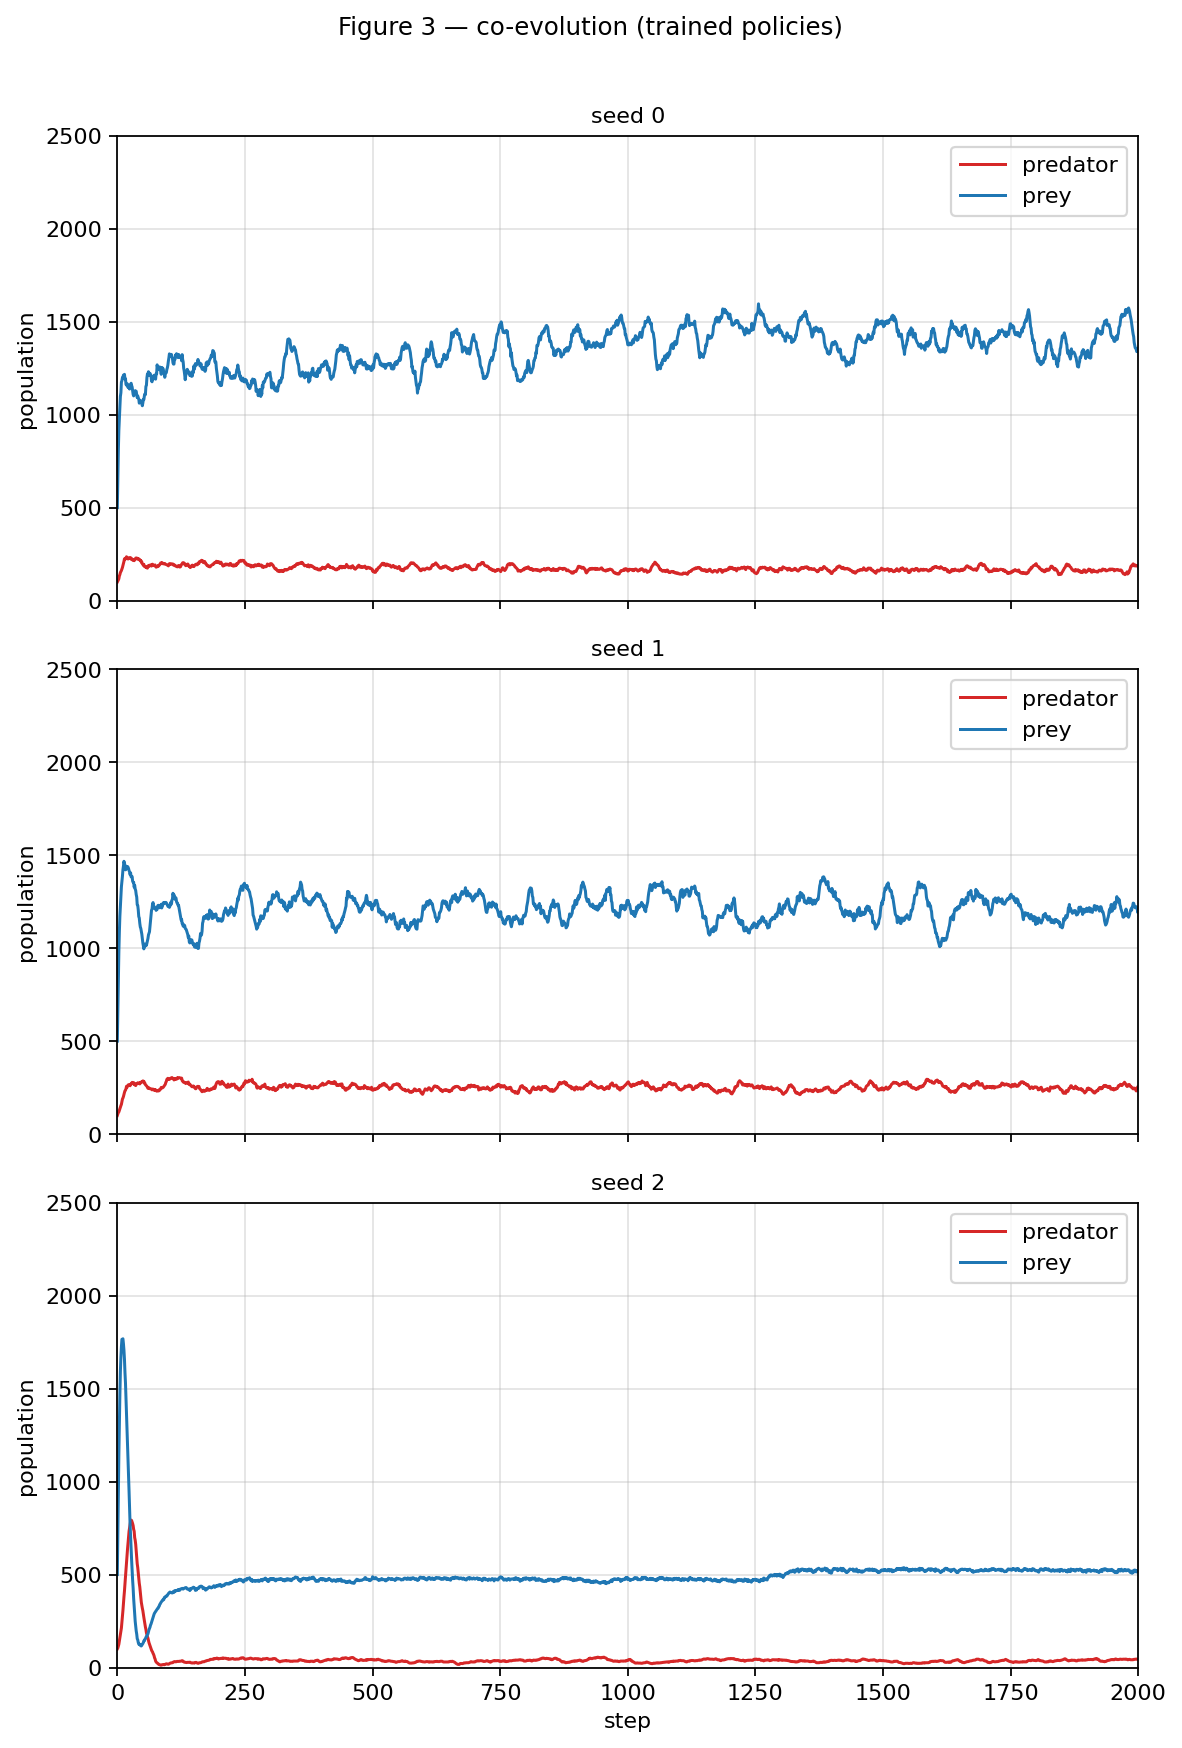
\includegraphics[width=0.95\textwidth]{../picks/figure3_co_evolution.png}
  \caption{Populacja drapieżników i ofiar przy \textbf{wytrenowanych} politykach po koewolucji (odpowiednik Fig.~3 w~\cite{park2021}). Trzy panele --- trzy ziarna losowe.}
  \label{fig:fig3}
\end{figure}

\begin{figure}[htbp]
  \centering
  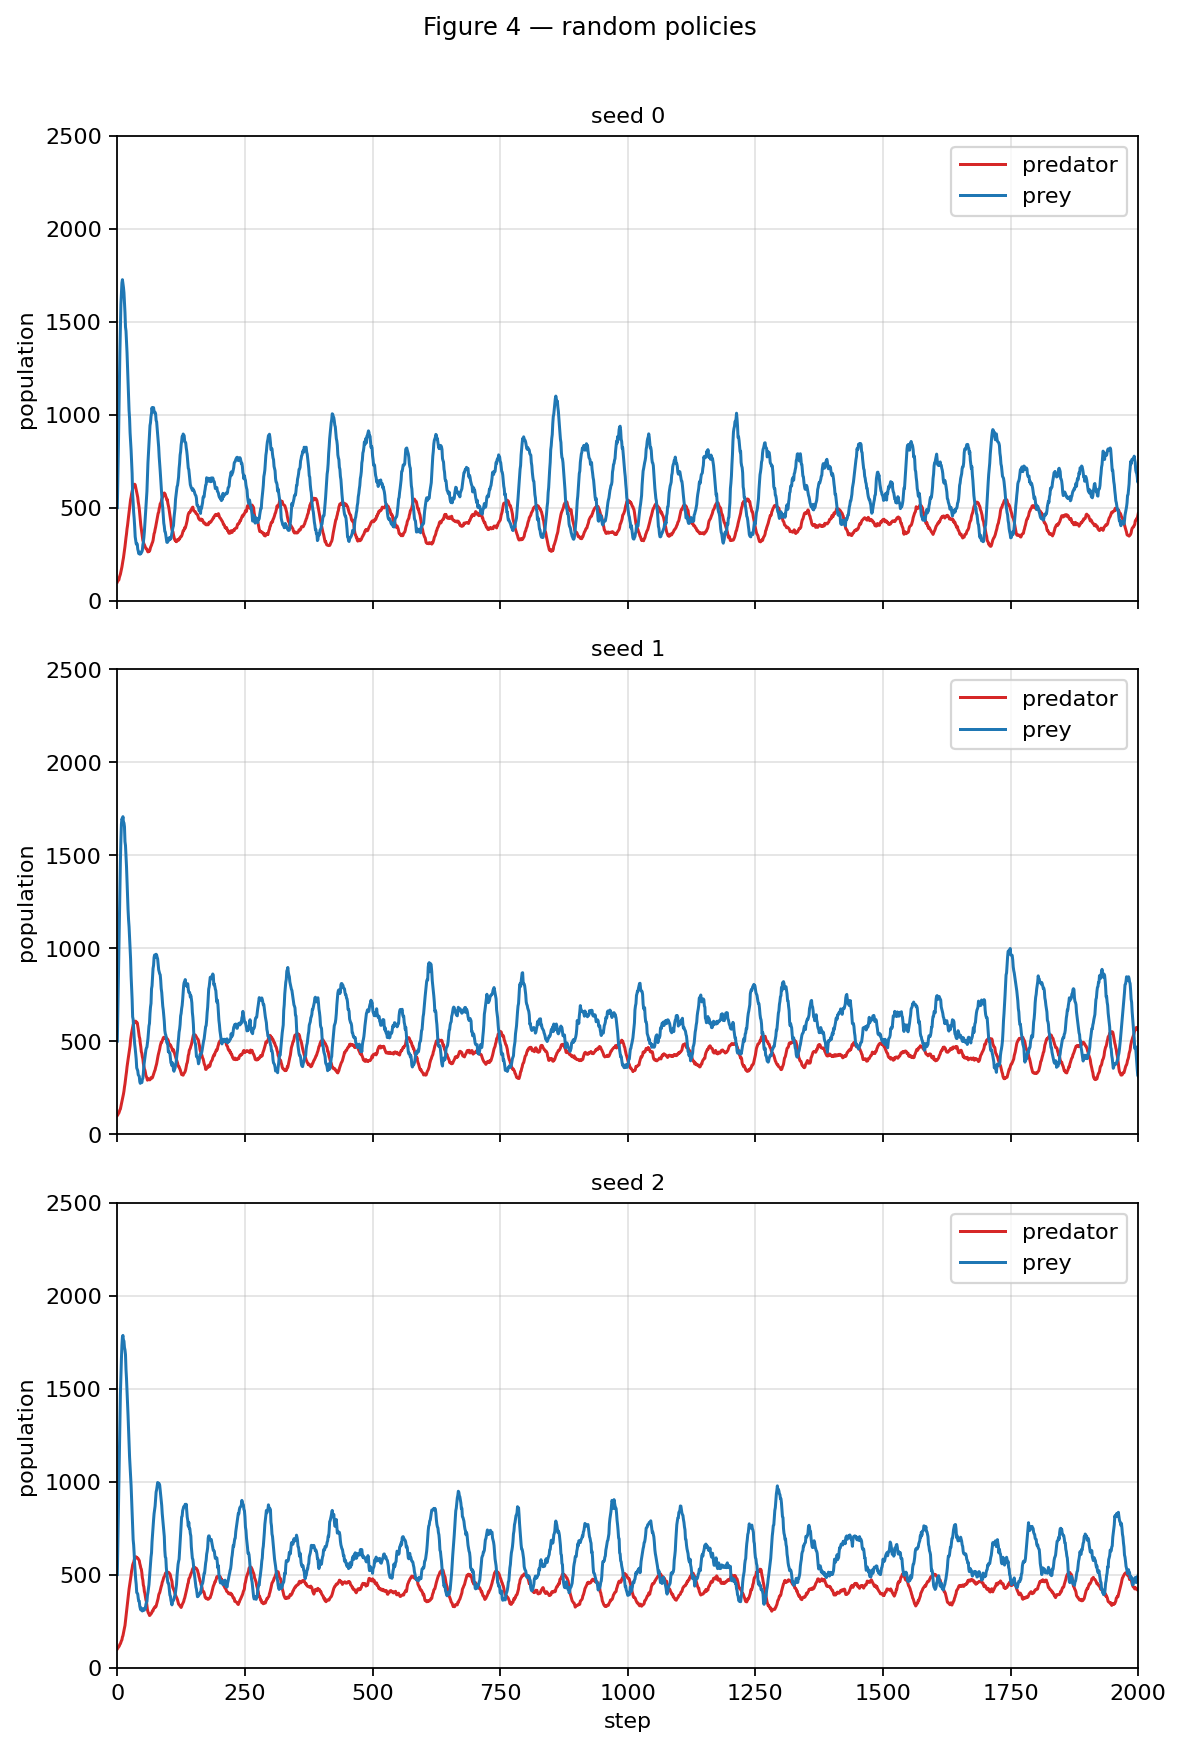
\includegraphics[width=0.95\textwidth]{../picks/figure4_random.png}
  \caption{Te same ustawienia osi i ziarna, lecz \textbf{jednostajnie losowe} akcje agentów --- linia bazowa (Fig.~4 w~\cite{park2021}).}
  \label{fig:fig4}
\end{figure}

\begin{figure}[htbp]
  \centering
  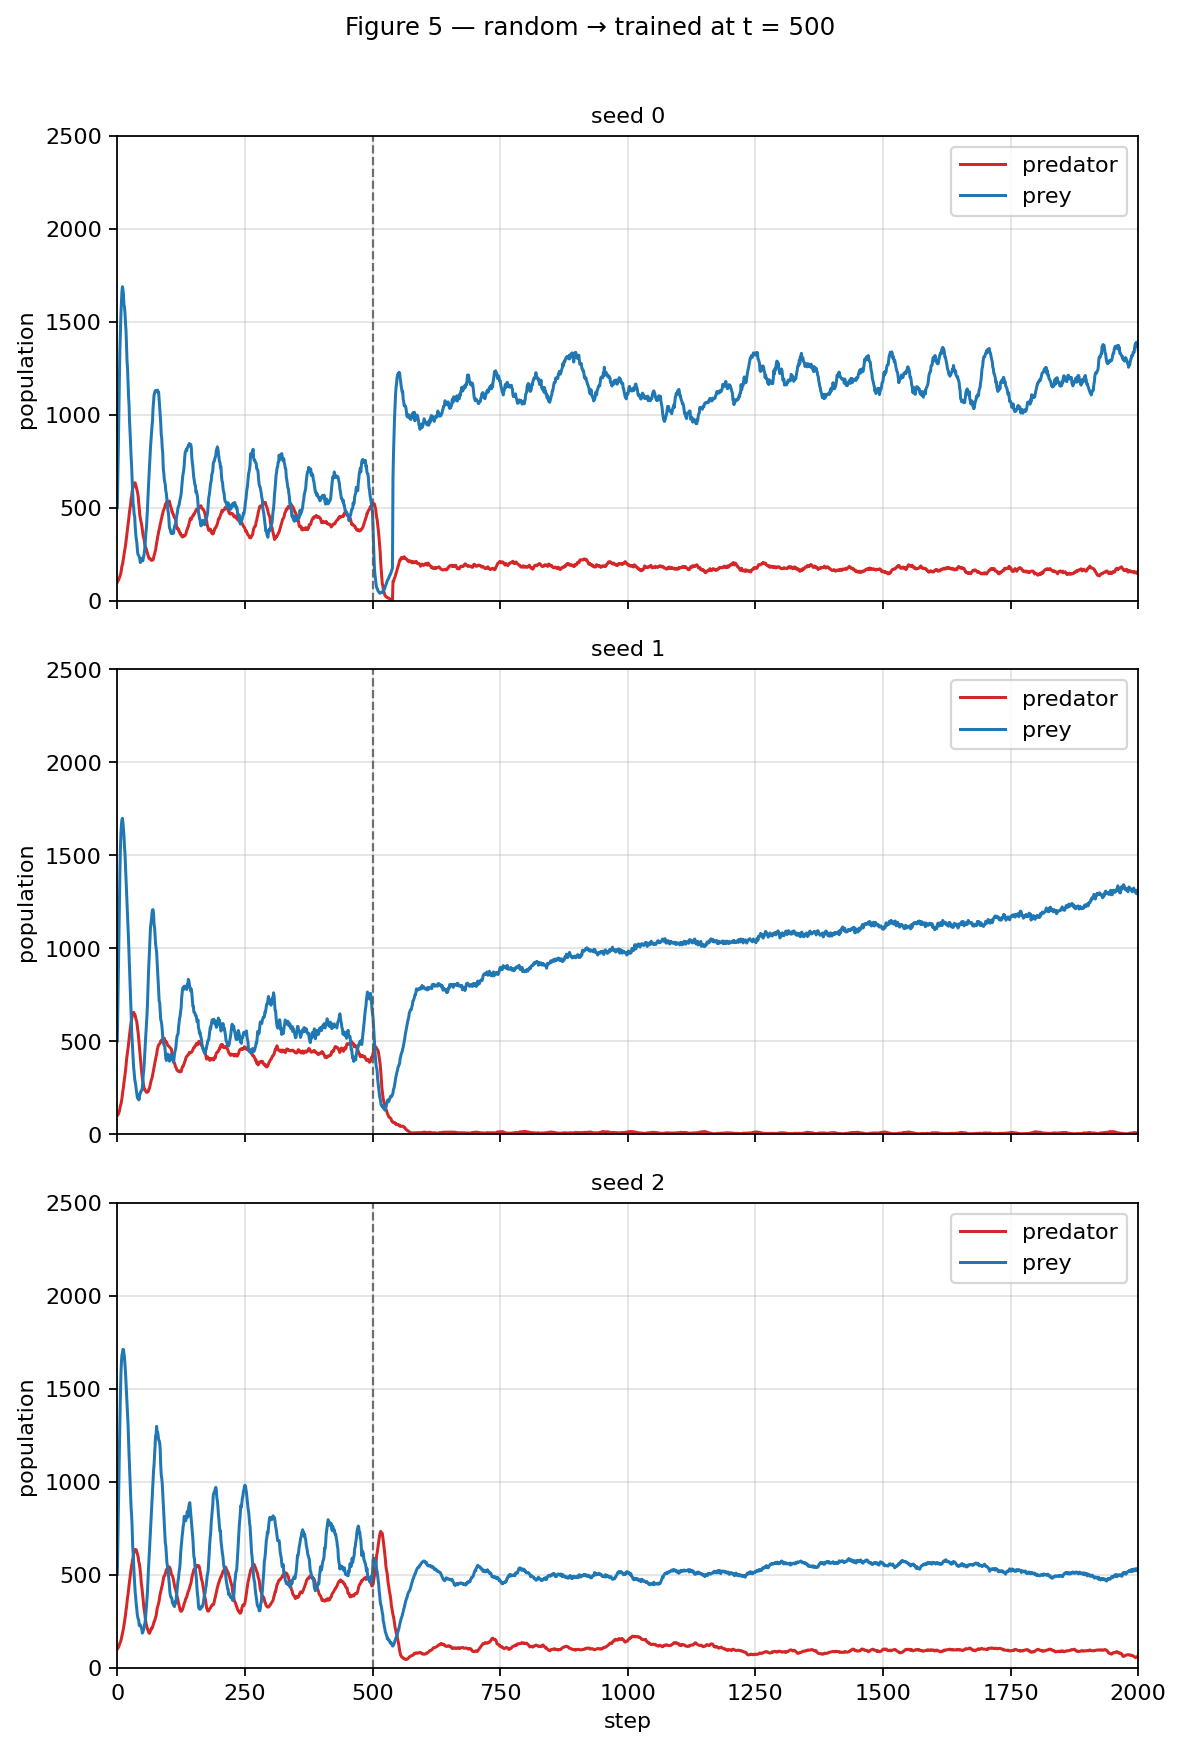
\includegraphics[width=0.95\textwidth]{../picks/figure5_random_then_trained.png}
  \caption{Pierwsze 500 kroków z losowymi akcjami, następnie polityki po uczeniu; pionowa linia przy \(t=500\) (Fig.~5 w~\cite{park2021}).}
  \label{fig:fig5}
\end{figure}

Na rys.~\ref{fig:fig3} widać, że po uczeniu przebiegi bywają stabilniejsze lub inaczej rozłożone niż przy polityce losowej (rys.~\ref{fig:fig4}), przy czym konkretny kształt oscylacji zależy od ziarna (np.\ gorszy reżim dla jednego z seedów). Rysunek~\ref{fig:fig5} ilustruje hipotezę z~\cite{park2021}: po przełączeniu na polityki wytrenowane dynamika często stabilizuje się po fazie dużych wahań; jednocześnie pojedyncze ziarna mogą prowadzić do niemal całkowitego wygaszenia drapieżników lub niskiej gęstości --- co podkreśla wrażliwość na stochastykę przy tej samej procedurze treningowej.

\subsection{Narzędzia eksperymentalne w repozytorium}
\label{sec:narzedzia}

\begin{itemize}
  \item \texttt{train\_park.py} --- interfejs CLI do pętli koewolucji; zapis wykresu populacji po iteracjach zewnętrznych (PNG/CSV), opcjonalnie podgląd Pygame.
  \item \texttt{reproduce\_paper\_figures.py} --- trening per ziarno oraz generacja rysunków typu Fig.~3--5 i plików CSV ze śladami kroków.
\end{itemize}

\subsection{Wnioski}
\label{sec:wnioski}

\begin{itemize}
  \item Implementacja odtwarza kluczowe elementy metody Park et al.~\cite{park2021}: częściowo obserwowalną grę na siatce z torusem, współdzielone polityki per gatunek, nagrody (\eqref{eq:nagrody-pred}--\eqref{eq:nagrody-prey}) oraz koewolucję z AlgaeDICE i horyzontem \(h=70\).
  \item Porównanie rys.~\ref{fig:fig3} i~\ref{fig:fig4} sugeruje, że uczenie ze wzmocnieniem zmienia jakościowo dynamikę populacji względem losowej polityki, zgodnie z intencją pracy źródłowej.
  \item Eksperyment z rys.~\ref{fig:fig5} pokazuje behawioralne przejście od eksploracji losowej do polityk uczenia --- z różnym skutkiem dla różnych ziaren, co warto traktować jako ograniczenie pojedynczego treningu bez dodatkowej selekcji hiperparametrów.
  \item Ograniczenia repozytorium względem pełnej pracy~\cite{park2021}: brak gotowej reprodukcji wszystkich rysunków jakościowych (np.\ trajektorie przestrzenne jak Fig.~6--7), deterministyczna kolejność ruchów agentów oraz domyślna liczba zewnętrznych iteracji (30) ustawiona pod wygodę eksperymentu, a nie identycznie z opisem ,,kilkudziesięciu'' iteracji w artykule.
\end{itemize}

\begin{thebibliography}{9}
\bibitem{park2021}
J.~Park, J.~Lee, T.~Kim, I.~Ahn, J.~Park.
\newblock Co-Evolution of Predator-Prey Ecosystems by Reinforcement Learning Agents.
\newblock \emph{Entropy} 2021, \emph{23}(4), 461.
\newblock \url{https://doi.org/10.3390/e23040461}
\end{thebibliography}

\end{document}
